\documentclass{standalone}
\usepackage{tikz}
\usepackage{ctex,siunitx}
\usepackage{tkz-euclide}
\usepackage{amsmath}
\usetikzlibrary{patterns, calc}
\usetikzlibrary {decorations.pathmorphing, decorations.pathreplacing, decorations.shapes,}
\begin{document}
\small
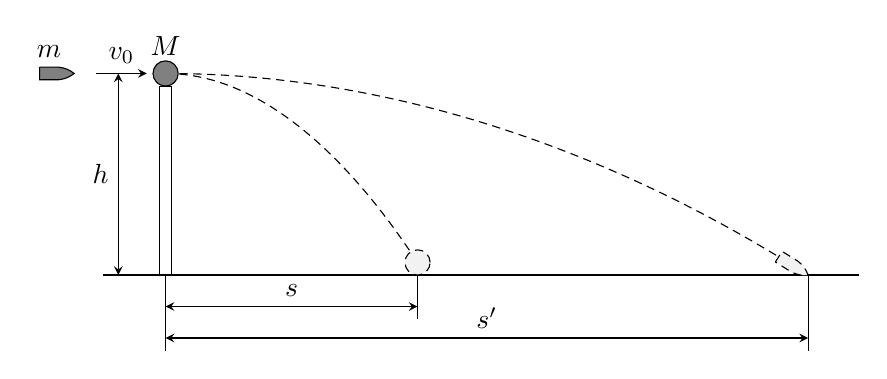
\begin{tikzpicture}[>=stealth,scale=0.8]
  \draw (-1,0)-- (11,0);
  \draw (-0.1,0) rectangle (.1, 3);
  \draw [<->](-.75,3.2)--node[left]{$h$}(-.75,0);
  \draw[fill=gray] (-2, 3.3) --(-1.7, 3.3)node[midway,above]{$m$} to [bend left=15] (-1.45, 3.2) to [bend left=15] (-1.7,3.1)--(-2,3.1)--(-2,3.3); 
  \draw[->](-1.1, 3.2)--node[above]{$v_0$}(-.3, 3.2);
  \draw [thin,<->](0,-.5)--node[above]{$s$}(4,-.5);
  \draw [thin,<->](0,-1.0)--node[above]{$s'$}(10.2,-1.0);
  \draw [thin](0,0)--(0,-1.2);
  \draw [thin](4,0)--(4,-.7);
  \draw [thin](10.2,0)--(10.2,-1.2);
  \draw [densely dashed] (0,3.2) parabola (4,0.2);
  \draw [densely dashed] (0,3.2) parabola (10.2,0);
  \draw [fill=gray] (0,3.2) circle (.2)node[above=1mm]{$M$};
  \draw [densely dashed,fill=gray!10] (4,.2) circle (.2);
  \begin{scope}[xshift=10.2cm]
  \draw [densely dashed,fill=gray!10,rotate=58] (-0.1,.55)--(0.1,.55)--(0.1,.25) to [bend left=15](0,0) to [bend left=15](-0.1,.25)--(-0.1,.55);
  \end{scope}
\end{tikzpicture}
\end{document}